\documentclass{standalone}


% Copy of relevant parts from the main preamble.
\usepackage{mathtools}

% Uncomment the following to use Times New Roman and Cambria Math
% \usepackage{unicode-math}
% \unimathsetup{math-style=TeX}
% \setmathfont[range=\mathup/{num}]{Times New Roman}
% \setmathfont[range=\mathit/{greek,Greek,latin,Latin}]{Cambria Math}
% \setmathfont[range=\mathup/{greek,Greek,latin,Latin}]{Cambria Math}
% \setmathfont[range={"2212,"002B,"003D,"0028,"0029,"005B,"005D,"221A,
% "2211,"2248,"222B,"007C,"2026,"2202,"00D7,"0302,"2261,"0025,"22C5,
% "00B1,"2194,"21D4,"2032}]
% {Cambria Math}
% \setmainfont[Ligatures=TeX]{Times New Roman}

% Uncomment the following to use Linux Libertine
% \usepackage[libertine]{newtxmath}
% \usepackage[no-math]{fontspec}
% \setmainfont{Linux Libertine O}

% Uncomment the following to use TeX Gyre Termes
% \usepackage{unicode-math}
% \unimathsetup{math-style=TeX}
% \setmainfont{TeX Gyre Termes}
% \setmathfont{TeX Gyre Termes Math}

% Uncomment the following to use TeX Gyre Pagella
\usepackage{unicode-math}
\unimathsetup{math-style=TeX}
\setmainfont{TeX Gyre Pagella}
\setmathfont{TeX Gyre Pagella Math}

% \usepackage[sfmath]{kpfonts}
% \renewcommand*\familydefault{\sfdefault}
% \usepackage[T1]{fontenc}

% \usepackage[no-math]{fontspec}
% Always use Inconsolata
\setmonofont{Inconsolata}

\usepackage{microtype}


\usepackage[version=3]{mhchem}
\usepackage{chemfig}
\setatomsep{2.25em}
\usetikzlibrary{positioning, calc, arrows.meta}
\tikzset{
    flux/.style={
        flux/.cd,
        #1,
        print,
    },
    flux/.cd,
    position/.store in=\position,
    position=0.6,
    fluxabove/.store in=\fluxabove,
    fluxbelow/.store in=\fluxbelow,
    print/.style={
        /tikz/.cd,
        insert path={%
            node [pos=\position, above] {\SI{\fluxabove}{\percent}} node[pos=\position, below] {\textbf{\SI{\fluxbelow}{\percent}}}%
        },
    },
}
\usepackage{siunitx}
\sisetup{detect-all=true}

\begin{document}
    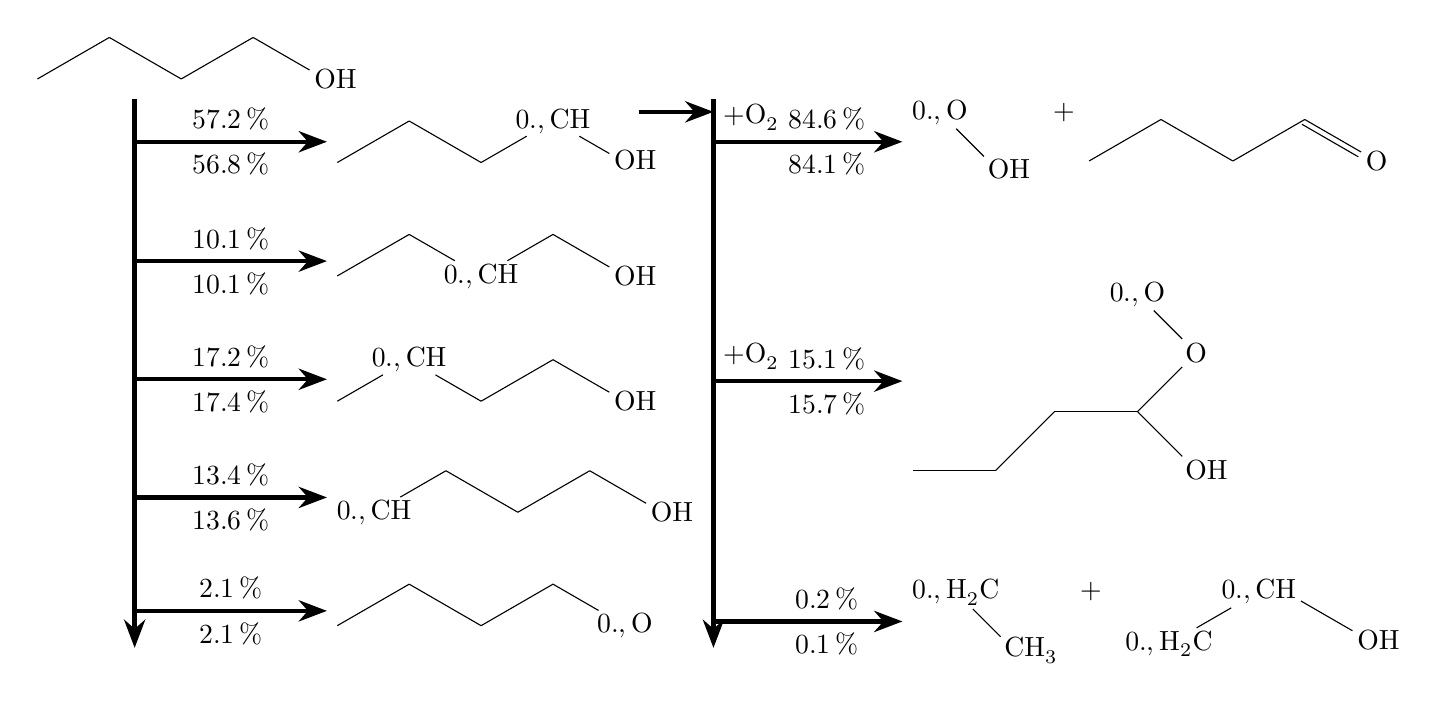
\begin{tikzpicture}[x=1cm, y=1cm]
        \begin{scope}[every node/.style={node distance=0.5}]
            \node (nbuoh) {\chemfig{-[:30]-[:330]-[:30]-[:330]OH}};
            \node[below right=0 and -0.5 of nbuoh] (anbuoh) {\chemfig{-[:30]-[:330]-[:30]\lewis{0.,CH}-[:330]OH}};
            \node[below left=0.5 and 0 of anbuoh, anchor=north west] (bnbuoh) {\chemfig{-[:30]-[:330]\lewis{0.,CH}-[:30]-[:330]OH}};
            \node[below left=0.5 and 0 of bnbuoh, anchor=north west] (gnbuoh) {\chemfig{-[:30]\lewis{0.,CH}-[:330]-[:30]-[:330]OH}};
            \node[below left=0.5 and 0 of gnbuoh, anchor=north west] (dnbuoh) {\chemfig{\lewis{0.,CH}-[:30]-[:330]-[:30]-[:330]OH}};
            \node[below left=0.5 and 0 of dnbuoh, anchor=north west] (onbuoh) {\chemfig{-[:30]-[:330]-[:30]-[:330]\lewis{0.,O}}};
            \node[right=3 of anbuoh] (nbuohalde) {\chemfig{\lewis{0.,O}-[7]OH} \, $+$ \,\chemfig[baseline=(c)]{-[:30]@{c}-[:330]-[:30]=_[:330]O}};
            \node[below left=1 and 0 of nbuohalde, anchor=north west] (anbuohoo) {\chemfig{--[1]-(-[7]OH)-[1]O-[3]\lewis{0.,O}}};
            \node[below left=1 and 0 of anbuohoo, anchor=north west] (scission) {\chemfig{\lewis{0.,H_2C}-[7]CH_3} \, $+$ \, \chemfig[baseline=(d)]{\lewis{0.,H_2C}-[:30,1.25]\lewis{0.,CH}@{d}-[:330]OH}};
        \end{scope}

        \begin{scope}[every path/.style={draw, ultra thick, >={Stealth}}]
            \path[->] let \p1 = (nbuoh.210), \p2 = (onbuoh.south) in (\x1,\y1) -- (\x1,\y2) coordinate (lineend);
            \path[->] ($(nbuoh.210)!(anbuoh)!(lineend)$) -- (anbuoh.west) [flux={fluxabove=57.2, fluxbelow=56.8, position=0.5}];
            \path[->] ($(nbuoh.210)!(bnbuoh)!(lineend)$) -- (bnbuoh.west) [flux={fluxabove=10.1, fluxbelow=10.1, position=0.5}];
            \path[->] ($(nbuoh.210)!(gnbuoh)!(lineend)$) -- (gnbuoh.west) [flux={fluxabove=17.2, fluxbelow=17.4, position=0.5}];
            \path[->] ($(nbuoh.210)!(dnbuoh)!(lineend)$) -- (dnbuoh.west) [flux={fluxabove=13.4, fluxbelow=13.6, position=0.5}];
            \path[->] ($(nbuoh.210)!(onbuoh)!(lineend)$) -- (onbuoh.west) [flux={fluxabove=2.1, fluxbelow=2.1, position=0.5}];
            \coordinate (midline) at ($(anbuoh.east)!0.2!(nbuohalde.west)$);
            \path[->] let \p1 = (anbuoh.north), \p2 = (midline), \p3 = (lineend) in (\x2,\y1) -- (\x2,\y3) coordinate (midlineend);
            \path[->, shorten <=-10] (anbuoh.10) -- ($(midline)!(anbuoh.10)!(midlineend)$);
            \path[->] ($(midline)!(nbuohalde)!(midlineend)$) -- (nbuohalde.west) [flux={fluxabove=84.6, fluxbelow=84.1}] node[pos=0.2, above] {$+$\ce{O2}};
            \path[->] ($(midline)!(anbuohoo)!(midlineend)$) -- (anbuohoo.west) [flux={fluxabove=15.1, fluxbelow=15.7}] node[pos=0.2, above] {$+$\ce{O2}};
            \path[->] ($(midline)!(scission)!(midlineend)$) -- (scission.west) [flux={fluxabove=0.2, fluxbelow=0.1}];
        \end{scope}
    \end{tikzpicture}
\end{document}
